\chapter{Telescopios ópticos}
Desde tiempos antiguos, el ser humano ha sido curioso y se ha permitido alzar la mirada al cielo, observando así diferentes cuerpos astronómicos, tales como el Sol, la Luna, los planetas del sistema solar e incluso las estrellas de nuestra Galaxia. Estos objetos nos brindan información crucial a través de la luz que emiten o reflejan, permitiéndonos estudiarlos desde la Tierra.

Para explorar las regiones más lejanas del universo, ha sido indispensable la construcción de telescopios; instrumentos que amplifican nuestra capacidad de observar y analizar regiones del espacio extremadamente distantes de nuestro planeta. Sin embargo, para aprovechar al máximo las observaciones astronómicas que estos telescopios nos proporcionan, es fundamental desarrollar una comprensión profunda de los principios de la luz, como su naturaleza, comportamiento y cómo interactúa con la materia.

\section{Telescopios}
\subsection{Naturaleza la luz}
En nuestra vida cotidiana, solemos referirnos a la luz como aquello que nuestros ojos pueden percibir. Sin embargo, gracias a la teoría del electromagnetismo y a las ecuaciones de Maxwell, entendemos que cuando partículas cargadas, como protones o electrones, se aceleran, generan ondas electromagnéticas. Estas ondas forman un vasto espectro conocido como el <<espectro electromagnético>>, del cual la luz <<óptica>> o <<visible>> constituye solo una pequeña porción. 

Las diferentes regiones del espectro electromagnético pueden ser descritas en términos de la longitud de onda, la frecuencia y la energía. La longitud de onda se mide en metros ($ m $) y se representa con el símbolo $ \lambda $ (letra griega lambda), mientras que la frecuencia se mide en unidades en hertz ($ \mathrm{1 Hz \equiv s^{-1}} $) y se representa con el símbolo $\nu$ (letra griega nu). Ambas cantidades se relacionan mediante:
\[ c = \lambda \nu, \]
donde $c$ es la velocidad de la luz en el espacio vacío y tiene un valor igual a $ 3\times 10^8 ~\mathrm{m ~ s^{-1}} $. La energía de la luz puede calcularse de manera simple con su frecuencia, gracias a la relación:
\[ E = h \nu, \]
donde $ h $ es la constante de Planck y tiene un valor numérico de $ 6.62607015\times 10^{-34} ~\mathrm{J~Hz^{-1}} $. Esta ecuación nos indica que a menor frecuencia (o de manera equivalente, a mayor longitud de onda), menor será la energía de la luz y viceversa.

La región óptica del espectro electromagnética está compuesta de luz cuya longitud de onda corresponde a todos los colores que percibimos, que van desde el azul ($ 420 \times 10^{-9} ~\mathrm{m} $) hasta el rojo ($ 640\times 10^{-9} ~\mathrm{m} $) y que pueden apreciarse en los arcoíris. En la Figura \ref{fig:em_spectrum} se muestra la región visible dentro de todo el espectro electromagnético.

\begin{figure}[htb]
  \centering
  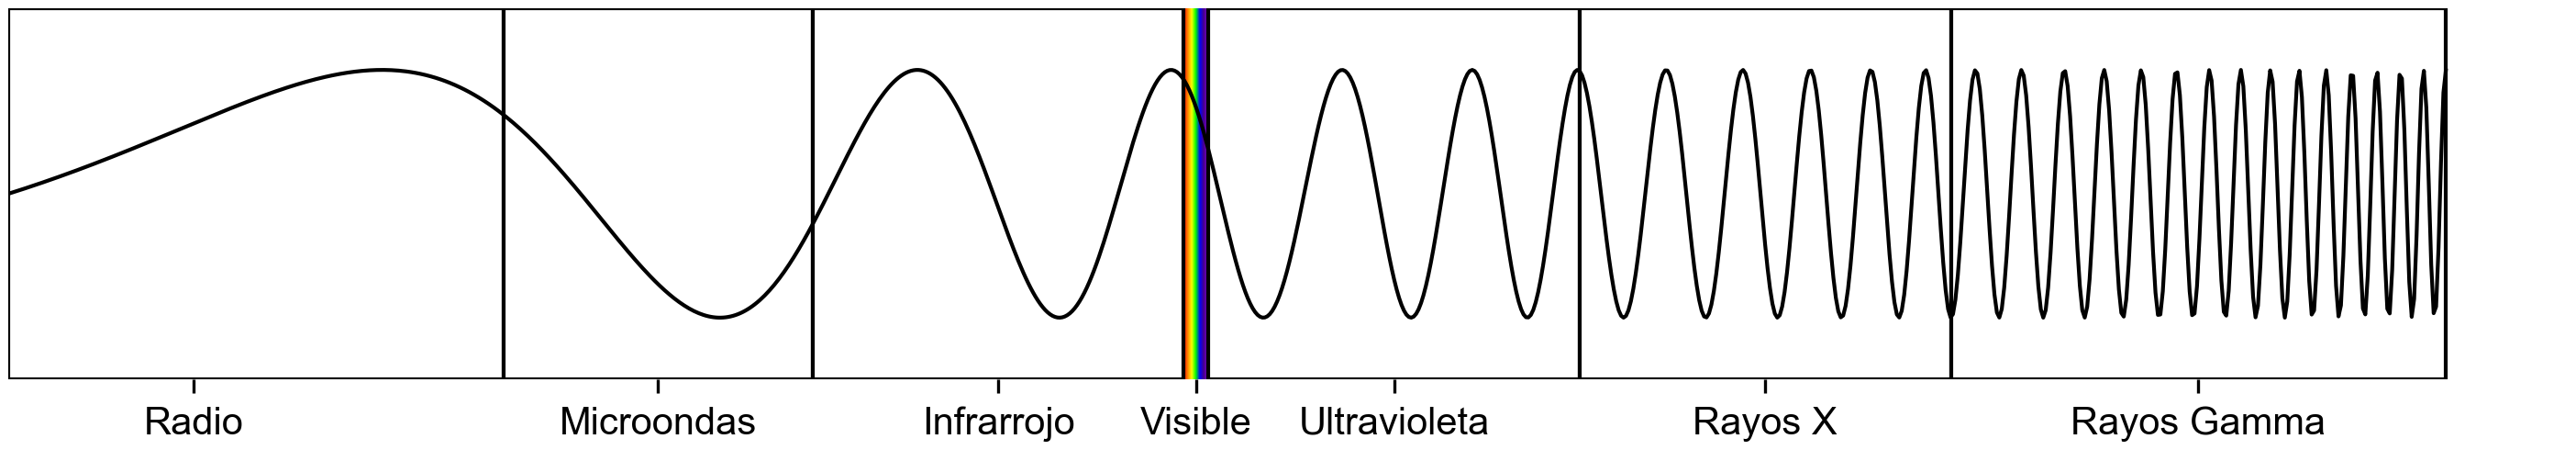
\includegraphics[width=\textwidth]{figures/em_spectrum.png}
  \caption{Espectro electromagnético}
  \label{fig:em_spectrum}
\end{figure}

Las diferentes porciones del espectro electromagnético reciben nombres específicos. Por ejemplo, la luz con longitudes de onda un poco más largas que el color rojo y que no somos capaces de ver se conoce como infrarrojo. Las ondas de radio son las ondas electromagnéticas con las longitudes de onda más largas y, por lo tanto, las menos energéticas. La región entre las ondas de radio y el infrarrojo se llama microondas, con longitudes de onda entre micrómetros y centímetros.

En el otro extremo del espectro, encontramos ondas electromagnéticas con longitudes de onda más cortas. Específicamente, la luz con longitud de onda más corta que el color violeta se llama ultravioleta. La luz con longitudes de onda aún menores se conoce como rayos X, y la luz con la longitud de onda más corta de todas se llama rayos gamma, que también es el tipo de radiación electromagnética más energética del universo.

\subsection{Principios básicos de óptica geométrica}
\subsection{Reflexión y refracción}
La óptica geométrica es una rama de la óptica que estudia y describe la luz en términos de rayos, donde un rayo se define como una línea imaginaria que indica la dirección en la que se propaga la luz. Esta dirección sigue un camino recto, permitiendo que la luz viaje entre dos puntos en el menor tiempo posible. Con esta aproximación de rayos, es posible describir la \textbf{refracción} y \textbf{reflexión} de la luz, los cuales son dos principios fundamentales que nos ayudarán a comprender cómo funcionan los telescopios. 

La refracción ocurre cuando la luz pasa a través de un material transparente, como el agua o el vidrio, mientras que la reflexión ocurre cuando la luz <<rebota>> sobre una superficie, como los espejos. Cuando la luz pasa de un material a otro (por ejemplo, del aire al agua), el camino que sigue la luz cambia de dirección, debido a que la velocidad de la luz es diferente en ambos medios. Para describir este cambio de dirección se utiliza la \textbf{Ley de Snell}:
\[ n_1 \sin\theta_1 = n_2 \sin \theta_2, \]
donde $ n_1 $ es el índice de refracción del primer material, $ n_2 $ es el índice de refracción del segundo material, $ \theta_1 $ es el ángulo incidente relativo a la normal de la superficie y $ \theta_2 $ es el ángulo de refracción relativo a la normal.

\begin{figure}[htb]
  \centering
  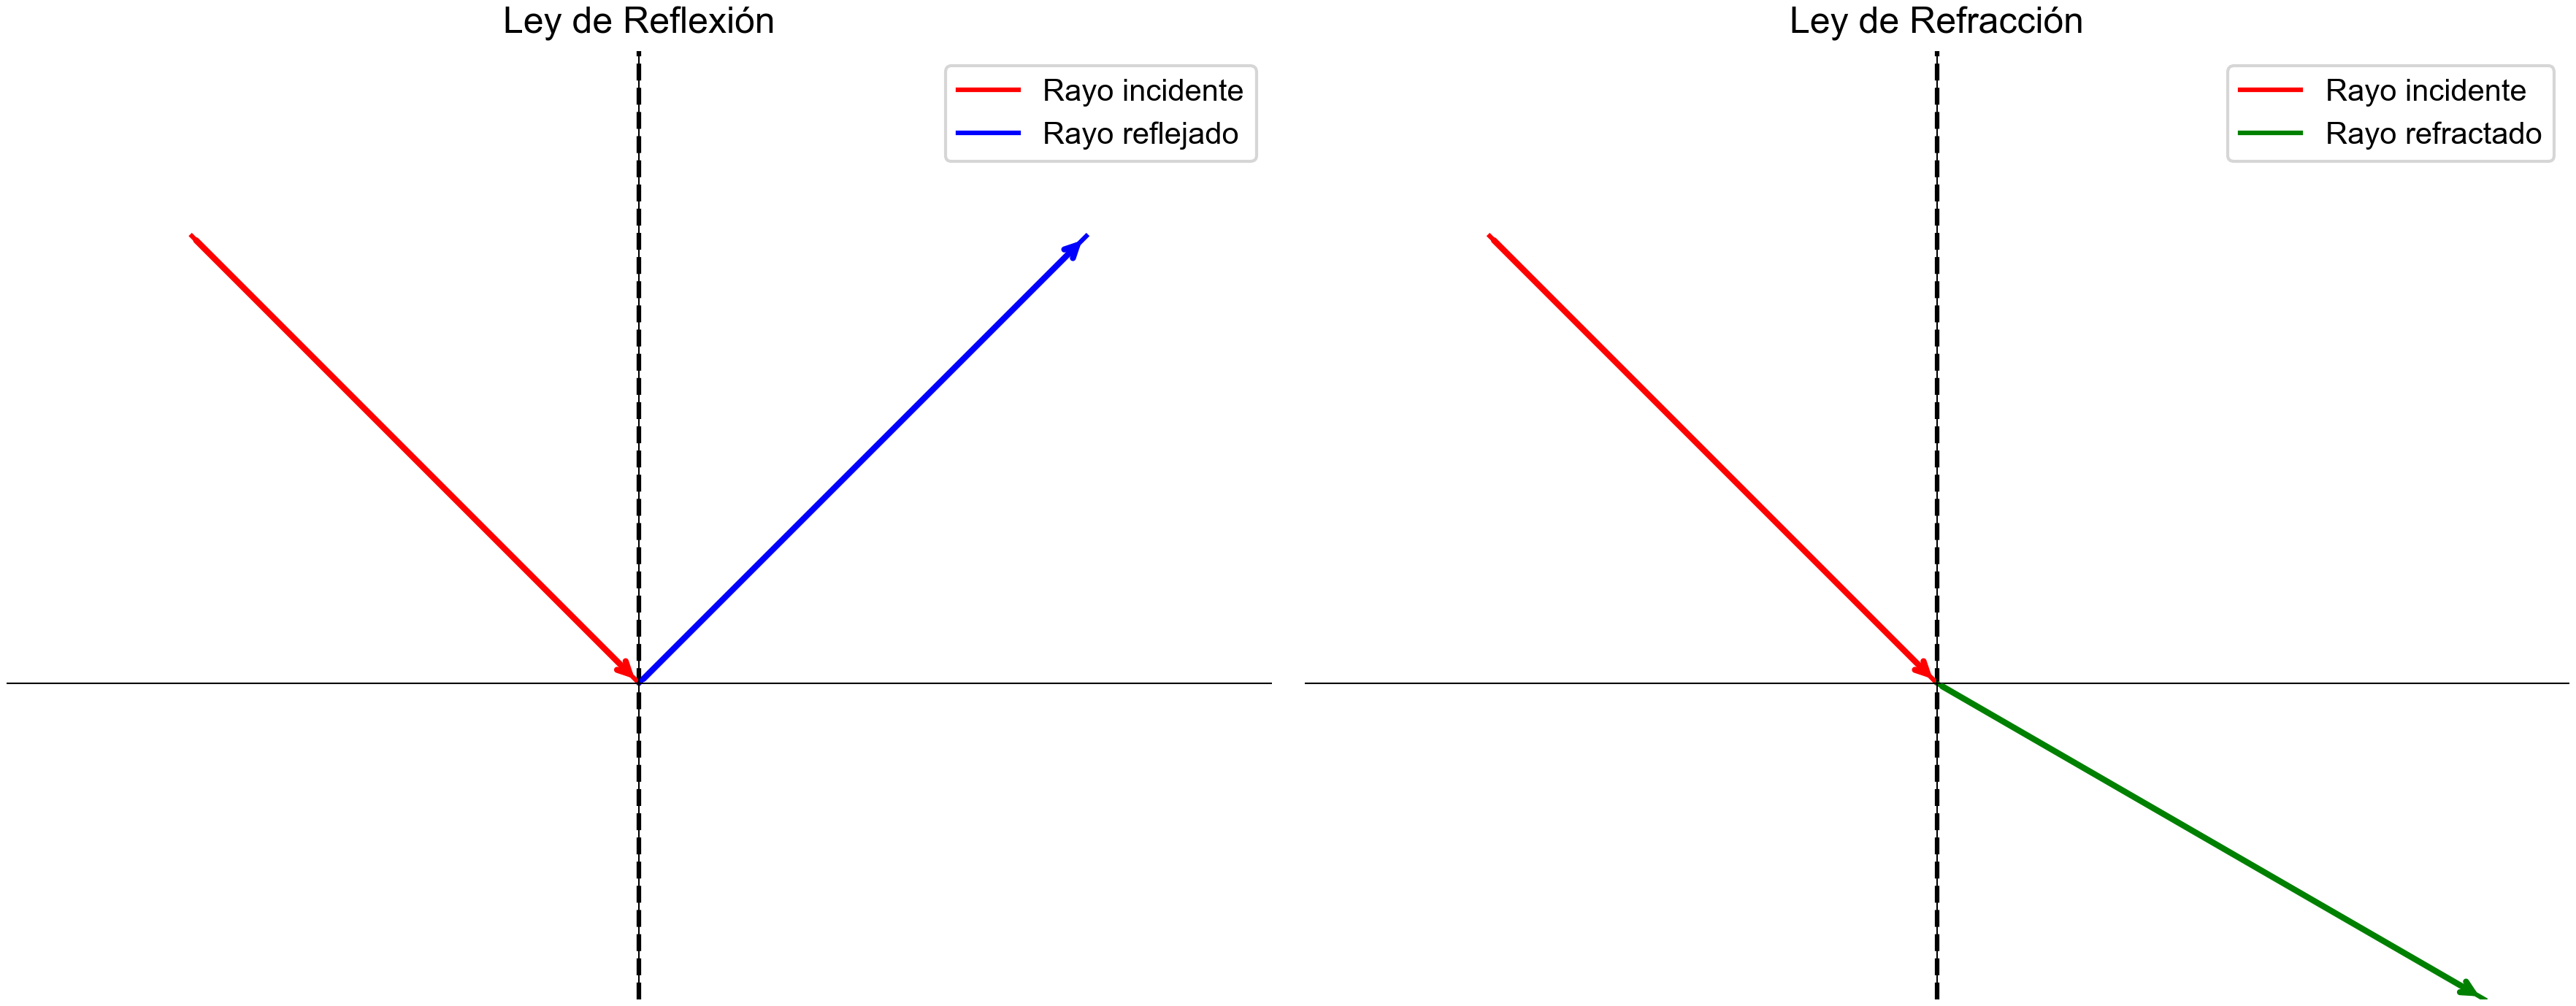
\includegraphics[width=\textwidth]{figures/light_laws.png}
  \caption{Leyes de refracción y reflexión}
  \label{fig:light_laws}
  \end{figure} 

El índice de refracción de un material es simplemente el cociente entre la velocidad de la luz en el vacío y la velocidad de la luz en ese material: $ n = c/v $. Como ejemplo, el índice de refracción del vidrio es 1.520, el del diamante es 2.417 y el del agua es 1.333.

Para superficies reflectivas, ocurre un principio aún más simple: el ángulo de incidencia es igual al ángulo de reflexión, para todas las longitudes de onda de la luz. Esta es conocida como la \textbf{ley de reflexión}. La ley de refracción y ley de reflexión se ilustran en la Figura \ref{fig:light_laws}.

\subsection{Propiedades de telescopios}
\subsubsection{Recolección de luz}
El principio de recolección de luz de los telescopios es bastante simple: mientras más grande sea el espejo o el lente, más luz coleccionará. La cantidad de luz recibida por unidad de tiempo es directamente proporcional al área de recolección y ya que la mayoría de los telescopios son circulares, esto significa que la proporción sigue la relación $ \pi r^2 $. 

